\documentclass[11pt]{article}

\usepackage[utf8]{inputenc}
\usepackage[margin=1in]{geometry}
\usepackage{amsmath,amssymb,amsthm}
\usepackage{mathtools}
\usepackage{booktabs}
\usepackage{graphicx}
\usepackage{microtype}
\usepackage[round,authoryear]{natbib}
\usepackage[colorlinks=true,linkcolor=blue!50!black,citecolor=blue!50!black,urlcolor=blue!50!black]{hyperref}
\usepackage{xcolor}
\usepackage{siunitx}
\sisetup{group-separator={,},group-minimum-digits=5}

\newtheorem{remark}{Remark}
\newcommand{\E}{\mathbb{E}}
\newcommand{\dd}{\mathrm{d}}
\newcommand{\ind}{\mathbf{1}}
\newcommand{\LB}{\mathrm{LB}}
\newcommand{\MLB}{\mathrm{MLB}}
\newcommand{\T}{\top}
\renewcommand{\labelitemi}{$\bullet$}

\title{Quintic B-spline collocation for continuously monitored\\ arithmetic Asian options under the Heston model}
\author{Mukhammad Sharif\\[2pt]
\small Astana IT University, Astana, Kazakhstan}
\date{October 2026}

\begin{document}
\maketitle

\begin{abstract}
We price continuously monitored, fixed-strike arithmetic Asian calls under the Heston model by solving
the two-dimensional pricing equation that results from the similarity reduction of Rogers, Shi and
Ve\v{c}e\v{r}. The equation is discretised in space by tensor-product quintic B-spline collocation and in
time by Crank--Nicolson with Rannacher start-up. Its coefficients do not depend on time, so a whole time
march costs two sparse LU factorisations, and one solve prices every strike. The degenerate boundary
$v=0$ needs no boundary condition: it is a collocation line on which the equation itself reduces to a
transport equation. To test the solver we build three references. The first is an exact price for the
geometric-average analogue, computed from a Riccati system. The second is the lower bound of Fusai and
Kyriakou, for which we derive the transform needed under Heston with a continuous average. The third is
a Monte Carlo estimator that uses this bound as a control variate and reaches a standard error of
$1.5\text{--}1.7\times10^{-5}$. On a parameter set that violates the Feller condition, the solver
agrees with this reference within its uncertainty at eleven strikes, and across thirteen parameter
regimes the standardised differences give $\chi^2=45.6$ for 39 comparisons. The time error is of second
order; in space the observed order approaches four from below, which is the limit set by collocation at
Greville points. At equal computing time the collocation error is about 150 times smaller than that of a
modified Craig--Sneyd ADI scheme on the same equation. Two side results concern practice. Truncating the
variance domain at $v_{\max}=1.5$ is harmless for vol-of-vol $\xi=1$ but moves the price by
$7\times10^{-4}$ at $\xi=1.5$, and grid refinement cannot detect this. We also could not reproduce the
published lower bounds for the Heston cases of Fusai and Kyriakou; we list the causes we can rule out.
\end{abstract}

\section{Introduction}\label{sec:intro}

An Asian option pays a function of the average price of its underlying over a fixed window. Averaging
makes the contract cheaper than its European counterpart and harder to manipulate near expiry, which is
why it is common on commodities and currencies. It also makes the contract harder to price. Even when the
underlying follows geometric Brownian motion, the arithmetic average of a lognormal process has no
tractable density, and the fixed-strike arithmetic Asian call has no closed-form price. For that model
the problem has been studied from many sides: the Laplace-transform formula of \citet{GemanYor1993} and
its extension to jump diffusions by \citet{CaiKou2012}, the spectral expansion of \citet{Linetsky2004},
and partial differential equation (PDE) methods, either on the full state space \citep{ZvanForsythVetzal1998}
or after the similarity reduction of \citet{RogersShi1995} and \citet{Vecer2001,Vecer2002}, which turns
the problem into a single space dimension. For continuous monitoring under geometric Brownian motion,
prices accurate to ten digits are available.

Under stochastic volatility the picture is thinner. In the \citet{Heston1993} model the variance is a
second state variable, the reduction of Rogers, Shi and Ve\v{c}e\v{r} leaves a two-dimensional PDE, and
the variance process may reach zero. \citet{FouqueHan2003} derived asymptotic approximations for fast
mean-reverting volatility. \citet{EwaldMenkensTing2013} obtained, through what they call the Australian
perspective, a two-dimensional pricing equation with time-independent coefficients and solved it with an
alternating direction implicit (ADI) finite difference scheme on a uniform grid, alongside Monte Carlo
schemes. \citet{FusaiKyriakou2016} developed optimised lower bounds for arithmetic Asian options in a
wide class of models and reported values for continuously monitored options under Heston. For the
geometric average under Heston, \citet{KimWee2014} gave a semi-closed-form price. For discrete monitoring
under stochastic volatility, transform and lattice-type methods are efficient
\citep{Corsaro2019,KirkbyNguyen2020}. \citet{PerottiGrzelak2024} extend Monte Carlo pricing of discretely
monitored Asian options under Heston with a data-driven sampling scheme and pay particular attention to
parameters that violate the Feller condition. \citet{CustersKarbachFriesen2026} derive semi-closed
formulas for discretely monitored Asian options in the rough Volterra--Heston model and use the geometric
price as a control variate for the arithmetic one. Recent work thus concentrates on discrete monitoring;
for the continuous case under Heston the published numbers are still mainly those of
\citet{EwaldMenkensTing2013} and \citet{FusaiKyriakou2016}. High-order discretisations of the Heston PDE exist as well, but
mainly for European and American options; a standard reference for the ADI side is
\citet{inthoutFoulon2010}.

What we did not find is a high-order solver for the continuously monitored arithmetic Asian option under
Heston whose accuracy has been checked against a reference fine enough to resolve it. The check matters
most in the case practitioners actually meet. Calibrated Heston parameters often violate the Feller
condition $2\kappa\theta\ge\xi^2$, so the variance reaches zero, the diffusion in the variance direction
degenerates on the boundary, and the solution may be less regular there. A method can converge smoothly
under refinement and still carry an error that refinement does not reveal; we meet two examples of this in
Section~\ref{sec:regimes}.

This paper offers such a solver together with the references needed to test it. The solver discretises
the reduced PDE with tensor-product quintic B-splines and collocates at Greville abscissae. Because the
coefficients of the reduced equation do not depend on time, a Crank--Nicolson march with Rannacher
start-up \citep{Rannacher1984} needs only two sparse LU factorisations, and since the strike enters only
through the point at which the solution is read, one solve prices all strikes. The boundary $v=0$, where
the Fichera theory forbids a boundary condition, is simply a line of collocation points on which the
equation degenerates by itself.

Most of the paper is about checking this solver. We use three references of increasing strength. The
first is the geometric-average version of the same contract, whose price we compute exactly (to about
$10^{-10}$) from a Riccati system; it shares the variance dynamics and the degenerate boundary with the
arithmetic problem and so tests the numerical machinery, though not the arithmetic reduction itself. The
second is the lower bound of \citet{FusaiKyriakou2016}. For Heston with a continuous average the transform
the bound requires is not given in that paper; we derive it by conditioning twice, which leads to two
consecutive Riccati systems, and validate the result independently. The third reference combines the two
previous ideas: the bound, being exact for the continuous average, serves as a control variate in a Monte
Carlo simulation, and the resulting estimator reaches a standard error of about $1.6\times10^{-5}$ with
no detectable time-discretisation bias. With this reference we compare the solver at eleven strikes and in
thirteen parameter regimes, measure its convergence in time and space, and compare it with the modified
Craig--Sneyd ADI scheme of \citet{inthoutFoulon2010} applied to the same equation.

Two findings came out of this checking and may be useful beyond this paper. First, the truncation of the
computational domain can produce errors that no refinement study will show, because refining the grid does
not move the boundary. A variance cut-off $v_{\max}=1.5$ is ample when the vol-of-vol is $\xi=1$ but
shifts the price by $7\times10^{-4}$ when $\xi=1.5$, and at a five-year maturity a cut-off $x_{\max}=8$
in the similarity variable shifts the at-the-money price by $3.5\times10^{-4}$. Only the independent reference exposed them.
Second, we could not reproduce the lower bounds that \citet{FusaiKyriakou2016} report for continuously
monitored options under Heston. Our bound is higher by up to $0.011$, a small amount in practical terms but
many standard errors of our simulation of the same quantity. We explain in Section~\ref{sec:published}
which causes we can exclude.

The paper is organised as follows. Section~\ref{sec:problem} states the problem, derives the reduced
equation and discusses its boundaries. Section~\ref{sec:method} describes the collocation scheme.
Section~\ref{sec:references} constructs the three references. Section~\ref{sec:results} reports the
numerical results, and Section~\ref{sec:conclusions} concludes. Appendix~\ref{app:transform} gives the
derivation of the transform used for the bound, and Appendix~\ref{app:tables} lists the numbers behind the
figures.

\section{Problem formulation}\label{sec:problem}

\subsection{Model and contract}

Under the pricing measure the asset price $S$ and its variance $v$ follow the \citet{Heston1993} dynamics
\begin{equation}\label{eq:heston}
\dd S_t = r S_t\,\dd t + \sqrt{v_t}\,S_t\,\dd W^{(1)}_t,\qquad
\dd v_t = \kappa(\theta - v_t)\,\dd t + \xi\sqrt{v_t}\,\dd W^{(2)}_t,\qquad
\dd\langle W^{(1)},W^{(2)}\rangle_t = \rho\,\dd t,
\end{equation}
with a constant short rate $r$ and no dividends. (A dividend yield only changes the drift of $S$ and can
be added without difficulty.) Let
\begin{equation*}
A_t = \int_0^t S_u\,\dd u
\end{equation*}
be the running integral of the price. The contract is the fixed-strike arithmetic Asian call with
continuous monitoring over $[0,T]$,
\begin{equation}\label{eq:price}
C(K) = e^{-rT}\,\E\Bigl[\Bigl(\tfrac{1}{T}A_T - K\Bigr)^{+}\Bigr].
\end{equation}

Unless stated otherwise we use the parameters of \citet[Table~2]{Corsaro2019}: $\kappa=1$, $\theta=0.09$,
$\xi=1$, $\rho=-0.3$, $v_0=0.09$, together with $S_0=100$, $r=0.04$ and $T=1$. For these values
$2\kappa\theta/\xi^2 = 0.18$, so the Feller condition fails by a wide margin. The stationary density of the
variance behaves like $v^{2\kappa\theta/\xi^2-1}=v^{-0.82}$ near zero: it is integrable, but it puts a lot
of mass close to the boundary, and the boundary is reached. This is the regime in which we want the solver
to be reliable, and in Section~\ref{sec:regimes} we move $\xi$, $\rho$ and $T$ around it.

\subsection{Similarity reduction}

A direct PDE formulation of \eqref{eq:price} has three space variables, $(S,A,v)$. The price is,
however, homogeneous of degree one in $(S,A,K)$, and following \citet{RogersShi1995} and
\citet{Vecer2001,Vecer2002} we write the time-$t$ value as
\begin{equation}\label{eq:ansatz}
V(t,S,A,v) = S\,w(t,x,v),\qquad x = \frac{K - A/T}{S}.
\end{equation}
Substituting \eqref{eq:ansatz} into the pricing equation for $V$, the terms $rV$ and $rS\,w$ cancel and
one is left with an equation for $w$ in two space variables,
\begin{equation}\label{eq:pde}
\frac{\partial w}{\partial t}
+ \tfrac12 v x^2 \frac{\partial^2 w}{\partial x^2}
- \rho\xi v x \frac{\partial^2 w}{\partial x\,\partial v}
+ \tfrac12 \xi^2 v \frac{\partial^2 w}{\partial v^2}
- \Bigl(r x + \frac1T\Bigr)\frac{\partial w}{\partial x}
+ \bigl(\kappa(\theta - v) + \rho\xi v\bigr)\frac{\partial w}{\partial v} = 0,
\end{equation}
with terminal condition
\begin{equation}\label{eq:terminal}
w(T,x,v) = \max(-x,0),
\end{equation}
since $(A_T/T-K)^+ = S_T\,(-x_T)^+$. At $t=0$ we have $A_0=0$, hence $x_0=K/S_0$ and
\begin{equation}\label{eq:readout}
C(K) = S_0\,w\bigl(0,\,K/S_0,\,v_0\bigr).
\end{equation}
\citet{EwaldMenkensTing2013} arrive at an equivalent equation through a change of measure to the stock
as num\'eraire; in that picture $w$ is a price in units of the stock, which explains why no discounting
term remains. Three properties of \eqref{eq:pde} shape everything that follows.

The first is that its coefficients do not depend on $t$. The discretised operator is therefore the same
at every time step, and any matrix factorisation can be reused for the whole time march.

The second is that the strike does not appear in \eqref{eq:pde}--\eqref{eq:terminal} at all. It enters
only through the point $x_0=K/S_0$ at which the solution is read in \eqref{eq:readout}, so one solution
prices all strikes whose $x_0$ lies inside the computational domain.

The third is that the equation contains the one-dimensional problem as a special case. If $\xi\to0$ and
$v_0=\theta=\sigma^2$, the variance stays at $\sigma^2$ and \eqref{eq:pde} becomes the Rogers--Shi
equation $w_t + \tfrac12\sigma^2x^2w_{xx} - (rx + 1/T)w_x = 0$ for geometric Brownian motion.

\subsection{Degeneracies and boundaries}\label{sec:boundaries}

\paragraph{The variance boundary $v=0$.} Every second-order term in \eqref{eq:pde} carries the factor $v$.
On $v=0$ the equation therefore reduces to the first-order equation
\begin{equation}\label{eq:v0}
\frac{\partial w}{\partial t} - \Bigl(rx+\frac1T\Bigr)\frac{\partial w}{\partial x} + \kappa\theta\,\frac{\partial w}{\partial v} = 0 .
\end{equation}
Since $\kappa\theta>0$, the drift of the variance points into the domain, and by the theory of equations
with nonnegative characteristic form \citep{OleinikRadkevich1973} no boundary condition may be imposed
on $v=0$; the value there is determined by the equation. For the Heston model this is the situation
analysed by \citet{EkstromTysk2010}. The practical consequence for a numerical method is that the
boundary line must carry the degenerate equation \eqref{eq:v0} itself, and not an artificial condition.
This holds whether or not the Feller condition is satisfied; what changes when it fails is how much
probability mass sits near the boundary.

\paragraph{The line $x=0$.} The diffusion coefficient $\tfrac12vx^2$ also vanishes on $x=0$, which is an
interior line of the domain, and the terminal condition \eqref{eq:terminal} has a kink there. The kink is
closer to the price than it looks. Along the drift alone, $x$ moves according to
$\dd x = -(rx+1/T)\,\dd t$, so that $x_T = (x_0 + 1/(rT))e^{-rT} - 1/(rT)$. For the at-the-money readout
$x_0=1$ and our parameters this gives $x_T\approx-0.02$: the characteristic through the readout point ends
almost exactly on the kink, in a region where the diffusion in $x$ is small.

\paragraph{Far field.} For $x\to-\infty$ the option is deep in the money and $w$ becomes linear in $x$;
for $x\to+\infty$ it is worthless. We truncate to $x\in[x_{\min},x_{\max}]$ and impose
\begin{equation}\label{eq:bcx}
\frac{\partial^2 w}{\partial x^2}(t,x_{\min},v) = 0,\qquad w(t,x_{\max},v) = 0 .
\end{equation}
For large variance we truncate at $v_{\max}$ and impose
\begin{equation}\label{eq:bcv}
\frac{\partial^2 w}{\partial v^2}(t,x,v_{\max}) = 0 .
\end{equation}
This condition allows $w$ to grow linearly in $v$ near the cut-off. In our tests it was much less sensitive
to the position of $v_{\max}$ than the more common $\partial w/\partial v=0$: at the base parameters,
moving $v_{\max}$ from $1.5$ to $4$ changed the at-the-money price by $7.0\times10^{-4}$ under the
Neumann condition and by $1.4\times10^{-6}$ under \eqref{eq:bcv} (at most $8\times10^{-6}$ over
$K=90,100,110$). The default domain is $x\in[-1,5]$,
$v\in[0,1.5]$. Section~\ref{sec:regimes} shows that this default has to be widened for some parameters.

\subsection{A geometric twin with an exact price}\label{sec:twin}

To test the numerical machinery against an exact answer we also solve the geometric-average version of
the contract,
\begin{equation*}
C_G(K) = e^{-rT}\,\E\bigl[(G_T - K)^+\bigr],\qquad G_T = \exp\Bigl(\frac1T\int_0^T \ln S_u\,\dd u\Bigr).
\end{equation*}
With $a(t) = (T-t)/T$ the variable
\begin{equation*}
\zeta_t = \frac1T\int_0^t \ln S_u\,\dd u + a(t)\ln S_t
\end{equation*}
satisfies $\dd\zeta_t = a(t)\bigl[(r - v_t/2)\,\dd t + \sqrt{v_t}\,\dd W^{(1)}_t\bigr]$; the term in
$\ln S_t$ cancels because $a'(t)=-1/T$. The price $u(t,\zeta,v)$ therefore solves
\begin{equation}\label{eq:pdegeo}
u_t + a(r - \tfrac v2)u_\zeta + \kappa(\theta-v)u_v + \tfrac12 a^2 v\,u_{\zeta\zeta} + \rho\xi a v\,u_{\zeta v}
+ \tfrac12\xi^2 v\,u_{vv} - r u = 0,\qquad u(T,\zeta,v) = (e^\zeta-K)^+,
\end{equation}
and $C_G(K) = u(0,\ln S_0,v_0)$. The variance part of \eqref{eq:pdegeo} is the same as in \eqref{eq:pde},
including the degeneracy at $v=0$, so the same boundary analysis applies. Two differences matter. The
coefficients now depend on time through $a(t)$, which we will see costs a factorisation per time step.
And the kink of the payoff lies at $\zeta=\ln K$, which for $K=S_0$ coincides with the readout point;
moreover the accumulated variance $\int_t^T a^2 v\,\dd s \approx v(T-t)^3/(3T^2)$ is cubically small near
maturity, so the kink is smoothed slowly. The geometric twin is thus a hard test of the time and space
discretisation, but it does not test the arithmetic reduction \eqref{eq:ansatz}. On the far boundaries we
use $u=0$ at $\zeta_{\min}$, the condition $u_{\zeta\zeta}-u_\zeta=0$ at $\zeta_{\max}$ (exact for any
function $Ae^\zeta+B$), and $u_v=0$ at $v_{\max}=4$.

\section{Quintic B-spline collocation}\label{sec:method}

\subsection{Spline spaces and grids}

We approximate $w(t,\cdot,\cdot)$ in a tensor-product space of quintic splines,
\begin{equation}\label{eq:tensor}
w(t,x,v) \approx \sum_{i=1}^{n_x}\sum_{j=1}^{n_v} c_{ij}(t)\,N_i(x)\,M_j(v),
\end{equation}
where $N_i$ and $M_j$ are B-splines of degree $p=5$ on open knot vectors (end knots repeated $p+1$ times)
\citep{deBoor2001}. The knots are the nodes of stretched grids. In each direction the nodes are
$y^\ast + \alpha\sinh(s)$ with $s$ uniform, so they cluster around a point $y^\ast$ with a width set by
$\alpha$. In $x$ we cluster around $x^\ast=0$ with $\alpha_x=0.3$: this is where the payoff has its kink
and where the $x$-diffusion vanishes. In $v$ we cluster around $v^\ast=0$ with $\alpha_v=0.15$.
For the convergence study of Section~\ref{sec:convergence} we fix the map exactly: the $s$-interval is
split at $s=0$ (the image of $x=0$) and the two sides receive $6k$ and $11k$ uniform steps, so that
$N_x = 17k+1$ and every grid in the sequence is an image of the same piecewise-linear map in $s$. Without
this precaution the number of nodes on each side of $x=0$ jumps by rounding from one grid to the next,
and the error constant jumps with it.

The payoff \eqref{eq:terminal} is only continuous at $x=0$, while a quintic spline with simple knots is
$C^4$. We insert $x=0$ as a knot of multiplicity four (removing any node closer than a quarter of the
local spacing), which makes the space $C^1$ there. A multiplicity of five would allow a kink in the
spline itself, but the second derivative would then be undefined at the kink, and a collocation method for
a second-order equation needs it. With multiplicity four the interpolant of the payoff is not exact, but
the error is confined to a few intervals around the kink.

The collocation points are the Greville abscissae $\xi_k = (t_{k+1}+\dots+t_{k+p})/p$ of each knot
vector. There are as many of them as there are basis functions, and they include both end points. In
particular $v=0$ is a collocation line.

\subsection{Collocation equations}

Let $B^{(d)}_x$ be the $n_x\times n_x$ matrix with entries $N_i^{(d)}(\xi_k)$, $d=0,1,2$, and define
$B^{(d)}_v$ in the same way. On the tensor grid of collocation points, and with $c$ the vector of
coefficients ordered by $x$ first, the values and derivatives of \eqref{eq:tensor} are
\begin{equation*}
M = B^{(0)}_x\otimes B^{(0)}_v,\quad
D_{xx} = B^{(2)}_x\otimes B^{(0)}_v,\quad
D_{xv} = B^{(1)}_x\otimes B^{(1)}_v,\quad
D_{vv} = B^{(0)}_x\otimes B^{(2)}_v,
\end{equation*}
and similarly $D_x$, $D_v$. Each one-dimensional matrix has at most six nonzeros per row, so the
Kronecker products have at most 36. Writing $\operatorname{diag}(f)$ for the diagonal matrix of a
coefficient $f$ evaluated at the collocation points, the spatial operator of \eqref{eq:pde} becomes
\begin{equation}\label{eq:Lh}
L = \operatorname{diag}\bigl(\tfrac12 v x^2\bigr)D_{xx} - \operatorname{diag}(\rho\xi v x)D_{xv}
+ \operatorname{diag}\bigl(\tfrac12\xi^2 v\bigr)D_{vv} - \operatorname{diag}\bigl(rx+\tfrac1T\bigr)D_x
+ \operatorname{diag}\bigl(\kappa(\theta-v)+\rho\xi v\bigr)D_v .
\end{equation}
The mixed derivative is simply one more sparse term; no splitting is involved.

Boundary conditions replace collocation equations. On the lines $x=x_{\min}$ and $x=x_{\max}$ and on
$v=v_{\max}$ the rows of \eqref{eq:Lh} are replaced by rows that evaluate \eqref{eq:bcx} or \eqref{eq:bcv}
with the exact derivatives of the basis functions. On $v=0$ nothing is replaced. There the diagonal
factors of the three second-order terms in \eqref{eq:Lh} are zero, and the remaining row is the
collocation of the degenerate equation \eqref{eq:v0}. The Fichera analysis of
Section~\ref{sec:boundaries} is thus built into the scheme without any special treatment, and the same
holds for the geometric twin.

\subsection{Time stepping}

In time-to-maturity $\tau=T-t$ the semi-discrete problem is $M\dot c = Lc$ (with boundary rows held at
their homogeneous values). We use the $\theta$-scheme
\begin{equation}\label{eq:theta}
(M - \theta\Delta\tau\,L)\,c^{n+1} = (M + (1-\theta)\Delta\tau\,L)\,c^n ,
\end{equation}
with four backward Euler steps ($\theta=1$) at the start and Crank--Nicolson ($\theta=\tfrac12$)
afterwards. The implicit start-up \citep{Rannacher1984} damps the high-frequency error created by the
kink; without it Crank--Nicolson is known to lose accuracy on non-smooth data
\citep{PooleyVetzalForsyth2003}. The initial coefficients $c^0$ are obtained by collocating the payoff,
$Mc^0 = w(T,\cdot,\cdot)$ at the collocation points, with the boundary rows included.

Since $L$ does not depend on $\tau$, the two matrices on the left of \eqref{eq:theta} are factorised once
each by a sparse LU decomposition, and each time step costs a sparse matrix--vector product and two
triangular solves. On the grid used for most results ($N_x=273$ nodes, $N_v=61$) the system has
$n_xn_v = 280\times65 = \num{18200}$ unknowns.

The error of Crank--Nicolson with Rannacher start-up behaves like
$c_2\Delta\tau^2 + c_3\Delta\tau^3 + \dots$; the cubic term comes from the four implicit steps, whose
local error is not symmetric in time. Where we need the time error to be negligible we therefore use two
levels of Richardson extrapolation,
\begin{equation}\label{eq:richardson}
R_1(\Delta\tau) = \frac{4P(\Delta\tau/2) - P(\Delta\tau)}{3},\qquad
R_2(\Delta\tau) = \frac{8R_1(\Delta\tau/2) - R_1(\Delta\tau)}{7},
\end{equation}
which needs three solves with $N_t$, $2N_t$ and $4N_t$ steps. Section~\ref{sec:convergence} confirms both
the second-order behaviour and the cubic remainder.

\subsection{Reading the price}

The price follows from \eqref{eq:readout} by evaluating the spline \eqref{eq:tensor} at
$(K/S_0, v_0)$:
\begin{equation*}
C(K) = S_0\sum_{i,j} c_{ij}\,N_i(K/S_0)\,M_j(v_0).
\end{equation*}
No interpolation between grid values is involved, and the evaluation is repeated for as many strikes as
needed at negligible cost. This removes a source of error that is easy to overlook with finite
differences, where the price at an off-grid point has to be interpolated and the interpolation error adds
to the discretisation error.

\subsection{The geometric twin}

The same construction applies to \eqref{eq:pdegeo}, with the kink knot at $\zeta=\ln K$. Its operator
depends on $\tau$ only through $a=\tau/T$ and splits as
\begin{equation*}
L(\tau) = a^2 M_2 + a M_1 + M_0 ,
\end{equation*}
where $M_2$ collects the $\zeta\zeta$ term, $M_1$ the $\zeta$ and $\zeta v$ terms and $M_0$ the rest. The
three matrices are assembled once, but the system matrix changes at every step and must be factorised
again. This is the main cost difference between the two problems and it matters for the comparison with
ADI in Section~\ref{sec:adi}.

\section{Reference values}\label{sec:references}

A published price accurate enough to test a high-order solver does not exist for this problem, so we
build our own. The three references below are independent of the collocation solver; how independent
they are of each other is discussed at the end of the section.

\subsection{Exact price of the geometric twin}\label{sec:geoexact}

Write $W^{(1)} = \rho W^{(2)} + \sqrt{1-\rho^2}\,W^{\perp}$ and let $Y_T = \frac1T\int_0^T\ln S_u\,\dd u$,
so that $G_T=e^{Y_T}$ and $Y_T=\zeta_T$. From the variance equation,
$\sqrt{v}\,\dd W^{(2)} = (\dd v - \kappa(\theta-v)\,\dd t)/\xi$, and integration by parts with $a(0)=1$,
$a(T)=0$ gives $\int_0^T a\,\dd v = -v_0 + \frac1T\int_0^T v\,\dd t$. The stochastic integral against
$W^{(2)}$ can therefore be written in terms of the variance path alone, and conditionally on that path
$Y_T$ is Gaussian. Its characteristic function is
\begin{equation}\label{eq:geochf}
\E\bigl[e^{iuY_T}\bigr] = \exp\bigl(iu\Lambda + \mathcal A(T) + \mathcal B(T)v_0\bigr),\qquad
\Lambda = \ln S_0 + \frac{rT}{2} - \frac\rho\xi\Bigl(v_0 + \frac{\kappa\theta T}{2}\Bigr),
\end{equation}
where, in time-to-maturity $\tau$ and with $a=\tau/T$,
\begin{equation}\label{eq:georiccati}
\frac{\dd\mathcal B}{\dd\tau} = \tfrac12\xi^2\mathcal B^2 - \kappa\mathcal B + c(\tau),\qquad
\frac{\dd\mathcal A}{\dd\tau} = \kappa\theta\mathcal B,\qquad \mathcal A(0)=\mathcal B(0)=0,
\end{equation}
\begin{equation*}
c(\tau) = iu\Bigl[-\frac a2 + \frac\rho\xi\Bigl(\frac1T + \kappa a\Bigr)\Bigr] - \frac{u^2}{2}(1-\rho^2)a^2 .
\end{equation*}
The Riccati equation has a time-dependent coefficient and we integrate it numerically (an eighth-order
Runge--Kutta method with relative tolerance $10^{-12}$), for all quadrature nodes at once. The price then
follows from the damped Fourier inversion of \citet{CarrMadan1999}, with damping $\alpha=1.5$ and
512 Gauss--Legendre nodes on $[0,200]$. The same representation underlies the semi-closed form of
\citet{KimWee2014}.

We checked this computation in three ways. In the limit $\xi\to0$, $\rho=0$, $v_0=\theta$ it reproduces the
Black--Scholes formula for the geometric Asian call with a relative error below $1.1\times10^{-11}$ for all
combinations of $r\in\{0,0.04,0.1\}$, $T\in\{0.25,1,5\}$ and dividend yield $q\in\{0,0.02\}$. For the full
model the price changes by less than $5\times10^{-11}$ when the damping is varied between $0.5$ and $3$ or
the quadrature is doubled, at maturities up to five years. And a direct simulation of the geometric payoff agrees with it within one standard error at every
maturity we tried ($T=0.25$, $3$ and $5$, two million paths each). For the base parameters
the prices are $13.3650818582$, $6.7095975217$ and $2.7174933218$ for $K=90$, $100$ and $110$.

\subsection{The lower bound of Fusai and Kyriakou under Heston}\label{sec:fk}

For any $\lambda\in\mathbb R$ the payoff satisfies $(A_T/T-K)^+ \ge (A_T/T-K)\,\ind\{Y_T>\lambda\}$, hence
\begin{equation}\label{eq:lb}
C(K) \ge \LB(\lambda) := e^{-rT}\,\E\bigl[(A_T/T-K)\,\ind\{Y_T>\lambda\}\bigr]
\end{equation}
for every $\lambda$. The idea of conditioning the arithmetic average on the geometric one goes back to
\citet{Curran1994} and \citet{RogersShi1995}. \citet{FusaiKyriakou2016} maximise \eqref{eq:lb} over
$\lambda$, which gives the maximal lower bound $\MLB = \LB(\lambda^\ast)$ with
$\E[A_T/T \mid Y_T=\lambda^\ast]=K$, and compute it by Fourier inversion in $\lambda$. With a damping
$\delta>0$,
\begin{equation}\label{eq:Phi}
\Phi(u;\delta) = \int_{\mathbb R} e^{(iu+\delta)\lambda}\,\LB(\lambda)\,\dd\lambda
= \frac{e^{-rT}}{iu+\delta}\Bigl[\frac1T\int_0^T\varphi_t(u-i\delta)\,\dd t - K\,\varphi_0(u-i\delta)\Bigr],
\end{equation}
\begin{equation}\label{eq:phis}
\varphi_t(\upsilon) = \E\bigl[S_t\,e^{i\upsilon Y_T}\bigr],\qquad \varphi_0(\upsilon) = \E\bigl[e^{i\upsilon Y_T}\bigr],
\end{equation}
and $\LB(\lambda) = \frac{e^{-\delta\lambda}}{\pi}\int_0^\infty \mathrm{Re}\bigl[e^{-iu\lambda}\Phi(u;\delta)\bigr]\dd u$.
(In the notation of \citet{FusaiKyriakou2016}, $\varphi_t=\phi_{t,t,T}(-i/2,\cdot)$ and
$\varphi_0=\phi_{T,T,T}(0,\cdot)$; see their equation (46).) For L\'evy models they give $\varphi_t$ in
closed form. For affine stochastic volatility models with a continuous average they describe the route,
via the joint characteristic function of variance, log-price and its integral and iterated conditioning,
but do not give formulas.

For the Heston model we compute $\varphi_t$ as follows; the details are in
Appendix~\ref{app:transform}. Let $X=\ln S$ and $c=i\upsilon/T$, so that
$S_te^{i\upsilon Y_T} = \exp\bigl(X_t + c\int_0^TX_u\,\dd u\bigr)$. Conditioning first on
$\mathcal F_t$, the expectation of $\exp(c\int_t^TX_u\,\dd u)$ is exponential-affine in $(X_t,v_t)$. The
product with $e^{X_t}$ and $\exp(c\int_0^tX_u\,\dd u)$ is again exponential-affine, and a second
conditioning on $\mathcal F_0$ finishes the computation. In time-to-maturity $\tau$ both stages solve the
same system
\begin{equation}\label{eq:twostage}
\frac{\dd B_x}{\dd\tau} = c,\qquad
\frac{\dd B_v}{\dd\tau} = \tfrac12B_x^2 - \tfrac12B_x + \rho\xi B_xB_v + \tfrac12\xi^2B_v^2 - \kappa B_v,\qquad
\frac{\dd \mathcal A}{\dd\tau} = rB_x + \kappa\theta B_v ,
\end{equation}
starting from zero, except that $B_x$ jumps by one at $\tau=T-t$, where the factor $e^{X_t}$ enters.
Hence $B_x(\tau) = c\tau + \ind\{\tau\ge T-t\}$, and
\begin{equation*}
\varphi_t(\upsilon) = \exp\bigl(\mathcal A(T) + (1+i\upsilon)\ln S_0 + B_v(T)\,v_0\bigr).
\end{equation*}
The first stage, $\tau\in[0,T-t]$, is the same for every $t$ and is integrated once with output at the
required points; the second stage is integrated separately for each quadrature node in $t$. Both are
vectorised over the Fourier variable and integrated numerically, so no branch of a complex logarithm has
to be tracked. We use 48 Gauss--Legendre nodes in $t$, 1024 nodes in $u$ on $[0,U]$ with
$U = 40/\sqrt{\bar vT/3}$ and $\bar v=\max(v_0,\theta)$, and $\delta=1$. The maximum over $\lambda$ is found by
a bounded scalar search, which is cheap because $\Phi$ is computed once and each evaluation of
$\LB(\lambda)$ is a single weighted sum. One parameter set with three strikes takes a few seconds in
Python.

\begin{table}[t]
\centering
\caption{Reproduction of Table~10 of \citet{FusaiKyriakou2016}: maximal lower bound (MLB) for the
Gaussian model, obtained with the Heston machinery in the limit $\xi\to0$ ($\xi=10^{-9}$, $\rho=0$,
$v_0=\theta=\sigma^2$). The last column is Linetsky's spectral price from the same table, for scale.}
\label{tab:fk10}
\footnotesize\setlength{\tabcolsep}{4.5pt}
\begin{tabular}{ccccc cccc}
\toprule
$S_0$ & $K$ & $r$ & $\sigma$ & $T$ & MLB (FK) & MLB (ours) & difference & Linetsky price\\
\midrule
2   & 2 & 0.02   & 0.10 & 1 & 0.055985 & 0.05598508 & $+7.9\times10^{-8}$ & 0.0559860415\\
2   & 2 & 0.18   & 0.30 & 1 & 0.218366 & 0.21836625 & $+2.5\times10^{-7}$ & 0.2183875466\\
2   & 2 & 0.0125 & 0.25 & 2 & 0.172226 & 0.17222617 & $+1.7\times10^{-7}$ & 0.1722687410\\
1.9 & 2 & 0.05   & 0.50 & 1 & 0.193060 & 0.19305997 & $-2.6\times10^{-8}$ & 0.1931737903\\
2   & 2 & 0.05   & 0.50 & 1 & 0.246298 & 0.24629819 & $+1.9\times10^{-7}$ & 0.2464156905\\
2.1 & 2 & 0.05   & 0.50 & 1 & 0.306094 & 0.30609360 & $-4.0\times10^{-7}$ & 0.3062203648\\
2   & 2 & 0.05   & 0.50 & 2 & 0.349779 & 0.34977879 & $-2.1\times10^{-7}$ & 0.3500952190\\
\bottomrule
\end{tabular}
\end{table}

We validated the implementation in four independent ways before using it.
\begin{itemize}
\item Without the jump in $B_x$ and at $t=T$, the system \eqref{eq:twostage} computes $\varphi_0$, the
characteristic function of $Y_T$. The geometric reference of Section~\ref{sec:geoexact} computes the same
quantity by a different derivation (it eliminates the log-price through the variance path), and the two
agree to $1.3\times10^{-15}$ on five parameter sets, including $T=5$ and a nonzero dividend yield.
\item For $\upsilon=0$ the system must return $\E[S_t]=S_0e^{rt}$ exactly, which it does to machine
precision.
\item In the Gaussian limit, $\LB(\lambda)$ has a closed form, because $(X_t,Y_T)$ is jointly Gaussian.
Our Fourier values agree with it to about $10^{-13}$ for all $\lambda$ tested, and the maxima reproduce all
seven values of Table~10 of \citet{FusaiKyriakou2016} to the six printed digits
(Table~\ref{tab:fk10}).
\item For the Heston parameter sets of their Table~9, a direct Monte Carlo estimate of $\LB(\lambda^\ast)$
at our $\lambda^\ast$ agrees with our Fourier value within two standard errors in nine runs
(three step sizes per set, standard errors $1.4$--$5.4\times10^{-4}$).
\end{itemize}
The bound is also stable: changing $\delta$ between $0.25$ and $2$ or doubling either quadrature moved it
by at most $1.4\times10^{-10}$ in every parameter set where we tried it, far below the Monte Carlo
uncertainty. Fusai and Kyriakou also give an upper bound for the error of the MLB. We did not
compute it: it requires conditional second moments of the average, and the values they report for
discretely monitored Heston options, $0.013$ to $0.049$, are far wider than the accuracy we need.

\subsection{Monte Carlo with the bound as control variate}\label{sec:e8}

Since the bound is exact for the continuous average, it can be used to correct a simulation, an idea
already used by \citet[Section~5]{FusaiKyriakou2016}. Along each path the difference
\begin{equation}\label{eq:gap}
\begin{aligned}
D &= e^{-rT}\Bigl[(A_T/T-K)^+ - (A_T/T-K)\,\ind\{Y_T>\lambda^\ast\}\Bigr]\\
  &= e^{-rT}\Bigl[(A_T/T-K)^+\ind\{Y_T\le\lambda^\ast\} + (K-A_T/T)^+\ind\{Y_T>\lambda^\ast\}\Bigr]
\end{aligned}
\end{equation}
is nonnegative and small: it is the part of the payoff that the bound misses, and it is nonzero only on
paths where the geometric average points the wrong way. We estimate
\begin{equation*}
C(K) = \MLB + \E[D]
\end{equation*}
by simulating $\E[D]$ with the quadratic-exponential scheme of \citet{Andersen2008}, antithetic normals,
and the trapezoidal rule for $A_T$ and $Y_T$. The time-discretisation bias of this estimator is the bias
of $\E[D]$ alone, and since $D$ is small, so is its bias.

For the base parameters $\E[D]$ is $0.0043$, $0.0036$ and $0.0038$ for $K=90,100,110$. We ran seven
independent batches with 32, 64 (eight million paths each) and 128, 256, 512, 1024 and 2048 (four million
paths each) time steps. The batches are mutually consistent ($\chi^2$ of 1.2, 9.4 and 7.2 on six degrees
of freedom), and a weighted regression of the estimates on the step size gives slopes within $1.8$
standard errors of zero. We therefore pool them. The result, which we call the reference price
throughout, is shown in Table~\ref{tab:ref}; we quote it with an uncertainty of $\pm3\times10^{-5}$,
which also covers the difference between the pooled value and the intercept of the regression. On the same
paths, a control variate based on the exact geometric price \citep{KemnaVorst1990} leaves a standard
error eight to ten times larger. The geometric control variate is the usual choice for arithmetic Asian
options under stochastic volatility, used recently by \citet{CustersKarbachFriesen2026} for discrete
monitoring, so the gain from the bound may be of use beyond the continuous case, although we have not
tested that. An estimate of that kind from eight million paths with 512 steps, which
is how we computed the reference before the bound was available, is listed for comparison; it differs
from the new reference by $1.3$ to $1.6$ of its own standard errors.

\begin{table}[t]
\centering
\caption{Reference prices for the base parameters ($\kappa=1$, $\theta=0.09$, $\xi=1$, $\rho=-0.3$,
$v_0=0.09$, $S_0=100$, $r=0.04$, $T=1$). MC: pooled estimate $\MLB+\E[D]$ from 36 million QE paths.}
\label{tab:ref}
\small
\begin{tabular}{lccc}
\toprule
& $K=90$ & $K=100$ & $K=110$\\
\midrule
Maximal lower bound (Section~\ref{sec:fk}) & 13.755959 & 7.028864 & 2.963683\\
$\E[D]$ & 0.004338 & 0.003634 & 0.003811\\
Reference price $\MLB+\E[D]$ & 13.760297 & 7.032498 & 2.967494\\
\quad standard error & $1.7\times10^{-5}$ & $1.5\times10^{-5}$ & $1.7\times10^{-5}$\\
\quad intercept of regression in $\Delta t$ & 13.760288 & 7.032471 & 2.967472\\
Geometric control variate only, 8M paths & 13.759848 & 7.032017 & 2.967033\\
\quad standard error & $3.5\times10^{-4}$ & $3.2\times10^{-4}$ & $2.8\times10^{-4}$\\
\bottomrule
\end{tabular}
\end{table}

At long maturities $\E[D]$ is larger ($0.014$--$0.035$ for $T=3$ and $5$), and there its bias does become
visible: at $T=3$ the estimate with 256 steps differs from those with 1024 and 2048 steps by up to
$6\times10^{-4}$. For these maturities we use 1024 steps or more.

\paragraph{How independent are the references?} The Monte Carlo reference and the bound do not use the
collocation solver in any way, and the bound's main ingredient, $\varphi_t$, is validated against three
separate checks. They do share with the geometric reference the affine structure of the model, numerical
integration of Riccati equations and Fourier inversion, and the reference price in Table~\ref{tab:ref}
depends on the bound directly. What the solver is compared with is therefore independent of the solver, but
not of the affine machinery. In Section~\ref{sec:published} we add a simulation with a different
time-stepping scheme and no control variate at all, which shares nothing with our other computations except
the model.

\section{Numerical results}\label{sec:results}

All computations were done in Python with NumPy and SciPy (SuperLU for the sparse factorisations) on a
two-core virtual machine. Timings are wall-clock times of single runs and are meant for comparing methods
on the same machine, not as absolute benchmarks. Unless stated otherwise the arithmetic problem uses the
domain $x\in[-1,5]$, $v\in[0,1.5]$, and prices are given for $K=90,100,110$.

\subsection{The machinery on the geometric twin}\label{sec:geo}

Table~\ref{tab:geo} shows the error of the collocation solver for the geometric twin \eqref{eq:pdegeo}
against the exact price of Section~\ref{sec:geoexact}, with $N_t=1600$, $N_v=31$, $v_{\max}=4$ and
$\zeta\in[\ln S_0-3.5,\ln S_0+3.5]$, the $\zeta$-grid clustered around $\ln K$. At the money the error
falls from $1.6\times10^{-3}$ to $10^{-4}$, and the observed order on successive pairs of grids is $2.0$,
$2.1$, $2.0$ and $2.1$. This low order is caused by the payoff. Here the kink lies exactly at the readout
point, and the variance accumulated near maturity is cubically small (Section~\ref{sec:twin}), so the
kink is barely smoothed by the time the solution is read. The knot of multiplicity four keeps the error
constant small but does not restore the order. Smoothing the initial data
\citep{KreissThomeeWidlund1970,PooleyVetzalForsyth2003} is the standard remedy; we do not pursue it,
because the geometric problem serves here only as a test. Away from the money the errors are not
monotone on coarse grids, where the kink is poorly resolved, and reach $10^{-6}$ ($K=90$) and
$10^{-5}$ ($K=110$) on the finest grid.

\begin{table}[t]
\centering
\caption{Geometric twin: collocation price minus exact price, $N_t=1600$, $N_v=31$, $v_{\max}=4$.}
\label{tab:geo}
\small
\begin{tabular}{rccc}
\toprule
$N_\zeta$ & $K=90$ & $K=100$ & $K=110$\\
\midrule
21 & $+2.4\times10^{-4}$ & $+1.64\times10^{-3}$ & $+1.36\times10^{-3}$\\
31 & $+5.6\times10^{-4}$ & $+7.41\times10^{-4}$ & $-1.15\times10^{-4}$\\
41 & $+3.3\times10^{-4}$ & $+4.04\times10^{-4}$ & $-1.43\times10^{-4}$\\
61 & $+7.1\times10^{-6}$ & $+1.82\times10^{-4}$ & $-6.05\times10^{-5}$\\
81 & $+1.1\times10^{-6}$ & $+9.87\times10^{-5}$ & $+1.35\times10^{-5}$\\
\bottomrule
\end{tabular}
\end{table}

What this experiment establishes is that the machinery converges to an exact price: the stretched grids,
the Kronecker assembly, the Rannacher start and, in particular, the treatment of the degenerate boundary
$v=0$ with the Feller condition violated. It does not test the arithmetic reduction \eqref{eq:ansatz}; that
is the job of the next two subsections.

\subsection{Arithmetic prices against the reference}\label{sec:arith}

Table~\ref{tab:arith} compares the collocation prices with the reference of Table~\ref{tab:ref}. The
collocation values were computed on the finest grid of Section~\ref{sec:convergence} ($N_x=1599$,
$N_v=61$) with time extrapolation \eqref{eq:richardson}, and corrected for the remaining $v$-error by the
difference between $N_v=91$ and $N_v=61$ on a coarser grid (at most $1.4\times10^{-7}$). What remains of the
discretisation error is of order $10^{-8}$, far below the uncertainty of the reference, so the comparison
tests the formulation and the reference rather than the grid. The differences are $-0.13$, $+1.62$ and
$-0.07$ standard errors.

\begin{table}[t]
\centering
\caption{Collocation prices against the reference price of Table~\ref{tab:ref} (base parameters). Differences are computed from unrounded values.}
\label{tab:arith}
\small
\begin{tabular}{lccc}
\toprule
& $K=90$ & $K=100$ & $K=110$\\
\midrule
Collocation (converged) & 13.7602945 & 7.0325229 & 2.9674926\\
Reference $\MLB+\E[D]$ & 13.760297 & 7.032498 & 2.967494\\
Difference & $-2.2\times10^{-6}$ & $+2.5\times10^{-5}$ & $-1.2\times10^{-6}$\\
Difference / standard error & $-0.13$ & $+1.62$ & $-0.07$\\
\bottomrule
\end{tabular}
\end{table}

A comparison at three strikes can hide a pattern across strikes. Figure~\ref{fig:strikes} repeats it for
eleven strikes from 80 to 130, that is $x_0$ from $0.8$ to $1.3$, all read from a single solve ($N_x=392$,
$N_v=61$, time-extrapolated), against a separate reference run of 16 million paths. All eleven differences
lie within one standard error of the reference, their signs show no trend, and
$\chi^2=4.1$ for 11 degrees of freedom. The numbers are listed in Table~\ref{tab:strikes}. The part of the
price that the bound misses, $\E[D]$, stays between $0.0037$ and $0.0052$ over this range.

\begin{figure}[t]
\centering
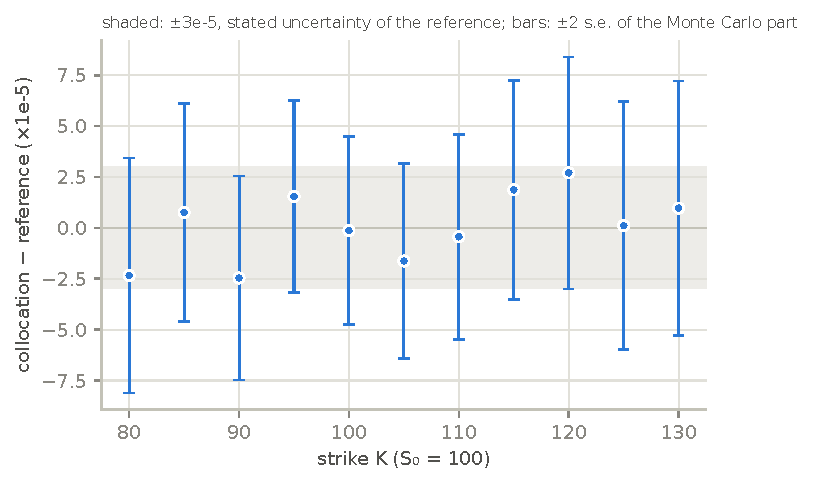
\includegraphics[width=0.78\textwidth]{figs/fig_strikes.pdf}
\caption{Collocation price minus reference price for eleven strikes (base parameters), in units of
$10^{-5}$. Bars show two standard errors of the Monte Carlo part of the reference; the shaded band is the
uncertainty $\pm3\times10^{-5}$ quoted for it.}
\label{fig:strikes}
\end{figure}

\subsection{Convergence in time and space}\label{sec:convergence}

\paragraph{Time.} We fix the spatial grid ($N_x=273$, $N_v=61$) and double the number of time steps from
800 to \num{25600}. Table~\ref{tab:time} shows the at-the-money price. Successive differences shrink by a
factor of $3.98$ to $4.00$, so the error is of second order. After one Richardson step the differences
shrink by a factor close to eight, which is the cubic term produced by the Rannacher steps. With two
levels of extrapolation over $N_t=1600,3200,6400$ the remaining time error, measured against the same
extrapolation over $6400,\dots,25600$, is below $5\times10^{-10}$ for the payoff and $5\times10^{-11}$ for a
smoothed terminal condition. For comparison, the time error of plain Crank--Nicolson with 1600 steps is
$1.5\times10^{-4}$ here, larger than the spatial error on this grid; the time step, not the grid, is what
limits a naive computation.

\begin{table}[t]
\centering
\caption{Time convergence of the at-the-money price ($K=100$, $N_x=273$, $N_v=61$). $d$: difference to
the previous row; $R_1$: one Richardson step \eqref{eq:richardson}; $d_{R}$: difference of $R_1$ to the
previous row.}
\label{tab:time}
\small
\begin{tabular}{rcccccc}
\toprule
$N_t$ & price & $d$ & ratio & $R_1$ & $d_R$ & ratio\\
\midrule
800   & 7.0331102118 & & & & &\\
1600  & 7.0326707632 & $-4.39\times10^{-4}$ & & 7.0325242803 & &\\
3200  & 7.0325604209 & $-1.10\times10^{-4}$ & 3.98 & 7.0325236401 & $-6.4\times10^{-7}$ &\\
6400  & 7.0325327736 & $-2.76\times10^{-5}$ & 3.99 & 7.0325235579 & $-8.2\times10^{-8}$ & 7.78\\
12800 & 7.0325258540 & $-6.92\times10^{-6}$ & 4.00 & 7.0325235474 & $-1.0\times10^{-8}$ & 7.89\\
25600 & 7.0325241231 & $-1.73\times10^{-6}$ & 4.00 & 7.0325235461 & $-1.3\times10^{-9}$ & 7.94\\
\bottomrule
\end{tabular}
\end{table}

\paragraph{Space.} With the time error removed in this way we refine the $x$-grid over ten levels,
$k=4,6,8,11,16,23,32,47,64,94$, which is $N_x$ from 69 to 1599 with the fixed map of
Section~\ref{sec:method}, and keep $N_v=61$. We estimate the order from three consecutive levels without a
reference solution: if $P(k)=P_\infty + Ck^{-q}$, the ratio of successive differences determines $q$. The
$v$-error does not affect these differences: repeating two levels with $N_v=91$ changes the differences by at
most $3\times10^{-10}$, while the differences themselves are $10^{-8}$ to $10^{-6}$.

To separate the effect of the kink we run two terminal conditions: the payoff \eqref{eq:terminal}, and the
smooth function $\frac12(\sqrt{x^2+\varepsilon^2}-x)$ with $\varepsilon=0.25$. Figure~\ref{fig:order} shows
the differences for $K=100$, and Table~\ref{tab:order} lists the last order estimates.

\begin{figure}[t]
\centering
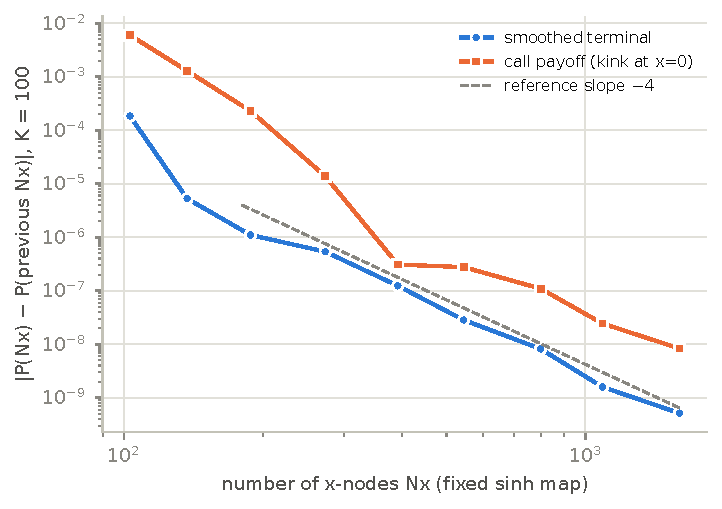
\includegraphics[width=0.78\textwidth]{figs/fig_order.pdf}
\caption{Spatial convergence at $K=100$: absolute difference between prices on consecutive $x$-grids,
plotted at the finer grid. Time error removed by two-level Richardson extrapolation; $N_v=61$.}
\label{fig:order}
\end{figure}

\begin{table}[t]
\centering
\caption{Spatial order estimated from three consecutive grids, for the last four triples (finest on the
right). Payoff estimates are shown only after the differences stop changing sign.}
\label{tab:order}
\small
\begin{tabular}{llcccc}
\toprule
terminal condition & $K$ & & & & finest\\
\midrule
smoothed & 90  & 3.80 & 3.90 & 3.96 & 3.96\\
smoothed & 100 & 3.94 & 3.97 & 3.99 & 3.99\\
smoothed & 110 & 2.11 & 3.43 & 3.72 & 3.92\\
payoff   & 90  & 3.60 & 3.80 & 3.91 & 3.96\\
payoff   & 100 & & 3.06 & 3.61 & 3.83\\
payoff   & 110 & & 2.79 & 3.56 & 3.82\\
\bottomrule
\end{tabular}
\end{table}

With the smooth terminal condition the estimates rise to $3.96$ and $3.99$ for $K=90$ and $100$ and still
move up for $K=110$. The observed order thus approaches four from below. This is what one should expect.
For maximally smooth splines of odd degree $p$, collocation at Greville points is known to converge more
slowly than Galerkin approximation in the same space \citep{Auricchio2010,Anitescu2015}. On a smooth
two-point boundary value problem, $-u''+u=f$ with $u=\sin\pi x$, our implementation converges in the
maximum norm at the rate $p-1$: $4.00$ for quintics and $2.00$ for cubics. We do not claim an
established order: the estimates are still increasing, and in our experience a rising slope is the
typical signature of a pre-asymptotic range.

With the actual payoff the behaviour is different at first. Between $N_x=69$ and $273$ the error falls from
$5$--$9\times10^{-3}$ to below $10^{-6}$, much faster than any fixed rate, and then the differences change
sign. After that the estimates climb towards four as well, reaching $3.82$ to $3.96$ on the finest grids.
At these resolutions the kink does not reduce the rate below that of the smooth problem. We have not
analysed why; a plausible reason is that the kink sits on the line $x=0$ while the price is read at
$x_0\approx1$, so that the local error of the payoff interpolation near $x=0$ is not the dominant term at
the readout point. On the geometric twin, where the kink coincides with the readout point, the picture is
different (Section~\ref{sec:geo}).

For practical purposes the relevant number is the size of the spatial error rather than its order. At
$N_x=273$ the difference to the finest grid is at most $7.3\times10^{-7}$ over the three strikes, forty times
smaller than the uncertainty of the reference.

\subsection{Parameter regimes and domain truncation}\label{sec:regimes}

We now leave the base parameters and vary one parameter at a time: $\rho\in\{-0.9,-0.7,0,0.5,0.9\}$,
$\xi\in\{0.3,0.6,1.5\}$ (Feller ratio $2\kappa\theta/\xi^2$ from $2.0$ down to $0.08$) and
$T\in\{0.25,0.5,3,5\}$. For each regime we compute a reference as in Section~\ref{sec:e8} (four million
paths and 256 steps for $T\le1$, with runs at 64 and 1024 steps added for $\rho=0.9$; 1024 and 2048 steps
pooled for $T\ge3$; the base set uses the reference of Table~\ref{tab:ref}) and a collocation price with
$N_x=392$, $N_v=61$ and time extrapolation.

The first pass through the regimes did not agree everywhere, and the disagreements are instructive. At
$\xi=1.5$ the collocation prices were above the reference by $6\times10^{-4}$ and $5\times10^{-4}$ for
$K=90$ and $100$, eight standard errors. We checked the reference first: the bound was unchanged to eight
digits under changes of damping and quadrature, and the Monte Carlo part showed no trend between 64, 256 and
1024 steps. On the solver side, refining $N_x$ or $N_v$ or changing the clustering changed the price by at
most $5\times10^{-6}$. Moving the variance cut-off from $v_{\max}=1.5$ to $3$ changed it by
$-7.2\times10^{-4}$, and moving it further to $5$ changed it by at most $5\times10^{-6}$. The cut-off was
the whole discrepancy. At the base value $\xi=1$ the same change of cut-off moves the price by less than
$10^{-5}$, which is why the default was adequate there. At $T=5$ we found the same kind of error at the
other end of the domain: moving $x_{\max}$ from 8 to 12 changed the price by $+2.7$ to $+4.4\times10^{-4}$,
while moving $x_{\min}$ or $v_{\max}$ changed it by less than $3\times10^{-5}$. Table~\ref{tab:trunc}
collects these tests.

\begin{table}[t]
\centering
\caption{Sensitivity of collocation prices to one change at a time, for the two regimes where the first
comparison failed and for $T=3$. Changes are new minus old price.}
\label{tab:trunc}
\small
\begin{tabular}{llccc}
\toprule
regime & change & $K=90$ & $K=100$ & $K=110$\\
\midrule
$\xi=1.5$ & $v_{\max}$: $1.5\to3$ & $-7.2\times10^{-4}$ & $-4.3\times10^{-4}$ & $-9.1\times10^{-5}$\\
          & $v_{\max}$: $3\to5$   & $-5.0\times10^{-6}$ & $-1.1\times10^{-6}$ & $+2.9\times10^{-6}$\\
          & $N_x$: $392\to545$     & $+1\times10^{-7}$   & $+7\times10^{-7}$   & $+4.8\times10^{-6}$\\
          & $N_v$: $61\to91$; clustering $\alpha_v$: $0.15\to0.05$ & $<10^{-7}$ & $<10^{-7}$ & $<10^{-7}$\\
$T=5$     & $x_{\max}$: $8\to12$  & $+2.7\times10^{-4}$ & $+3.5\times10^{-4}$ & $+4.4\times10^{-4}$\\
          & $x_{\min}$: $-2\to-3$ & $+2.6\times10^{-5}$ & $+1.3\times10^{-5}$ & $+7.3\times10^{-6}$\\
          & $x\in[-3,12]\to[-4,16]$ & $+3.9\times10^{-5}$ & $+6.1\times10^{-5}$ & $+8.0\times10^{-5}$\\
          & $v_{\max}$: $3\to5\to8$ & $<2\times10^{-5}$ & $<2\times10^{-5}$ & $<2\times10^{-5}$\\
$T=3$     & $v_{\max}$: $3\to5\to8$ & $<4\times10^{-6}$ & $<4\times10^{-6}$ & $<4\times10^{-6}$\\
          & $x\in[-2,8]\to[-3,12]$ & $+2.7\times10^{-5}$ & $+3.7\times10^{-5}$ & $+4.9\times10^{-5}$\\
\bottomrule
\end{tabular}
\end{table}

Neither error can be found by refining the grid, because refinement does not move the boundary: the
solutions converged smoothly, just to a slightly wrong limit. Both were found only because an independent
reference was available at the $10^{-5}$ level. We draw a practical conclusion: in the Heston setting the
truncation of the domain has to be checked separately for each parameter regime, by moving the boundary,
and the default that works at one parameter set does not transfer. Heavier vol-of-vol spreads the
variance distribution, and longer maturities spread the similarity variable.

After widening the domain where needed ($v_{\max}=3$ for all regimes with $T\le1$; $x\in[-3,12]$ at $T=3$;
$x\in[-4,16]$ with $N_x=545$ at $T=5$), the comparison is shown in Figure~\ref{fig:regimes}, with the
numbers in Table~\ref{tab:regimes}. Of the 39 standardised differences, 38 lie within two standard errors,
and their sum of squares is $\chi^2=45.6$ for 39 degrees of freedom. The one exception is $\rho=0.9$,
$K=90$, at $+2.9$ standard errors. There the grid matters: going from $N_x=392$ to $545$ moved this price by
$-4.6\times10^{-5}$, the largest refinement effect we saw, and the value shown is already the finer one.
With strong positive correlation the mixed term $-\rho\xi vx\,w_{xv}$ is large and the solution needs finer
$x$-resolution. The standard errors of the references range from $6\times10^{-6}$ at $T=0.25$ to
$1.9\times10^{-4}$ at $T=5$.

\begin{figure}[t]
\centering
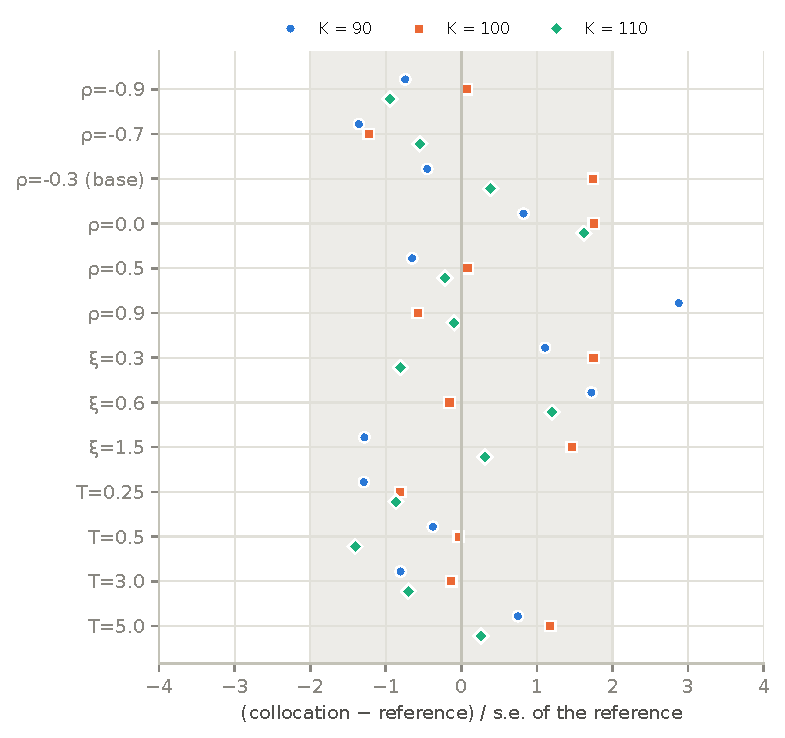
\includegraphics[width=0.72\textwidth]{figs/fig_regimes.pdf}
\caption{Collocation minus reference, divided by the standard error of the reference, for thirteen
parameter regimes and three strikes. One parameter is changed at a time from the base set ($\rho=-0.3$,
$\xi=1$, $T=1$). The shaded band is $\pm2$.}
\label{fig:regimes}
\end{figure}

\subsection{Comparison with ADI}\label{sec:adi}

To compare with a standard method we implemented the modified Craig--Sneyd ADI scheme of
\citet{inthoutFoulon2010} for the same equation \eqref{eq:pde}, on the same domain and with the same
boundary conditions: second-order central differences on stretched grids clustered at $x=0$ and $v=0$,
a second-order one-sided difference in $v$ on the degenerate boundary, $\theta=1/3$, four Rannacher steps,
and bicubic interpolation for the readout. Because the coefficients do not depend on time, all
factorisations of the ADI stages are also computed once, outside the time loop. Without this the
comparison would be unfair to ADI.

Figure~\ref{fig:comparator} plots the largest error over the three strikes against the time for one solve
(each solve prices all three strikes, for both methods). The error is measured against the converged
collocation price, which agrees with the reference within its uncertainty
(Section~\ref{sec:arith}); using the reference itself would cut off the collocation curves at
$3\times10^{-5}$. Plain Crank--Nicolson collocation reaches an error of $10^{-3}$ in about two seconds and
$10^{-4}$ in about eight. With two levels of extrapolation in time it reaches $2\times10^{-5}$ in 14 seconds
and $7\times10^{-7}$ in 76 seconds. ADI needs 25 seconds for $5\times10^{-3}$ on a $961\times121$ grid, and its
error falls roughly like $t^{-1.3}$ with the computing time $t$. At an equal cost of about three seconds
the collocation error is about 150 times smaller. On the finer ADI grids the error at $K=110$ is $1.4$ to $1.8$
times the error at the money, so a comparison at $K=100$ alone understates the difference. The individual runs are
listed in Table~\ref{tab:comp}.

\begin{figure}[t]
\centering
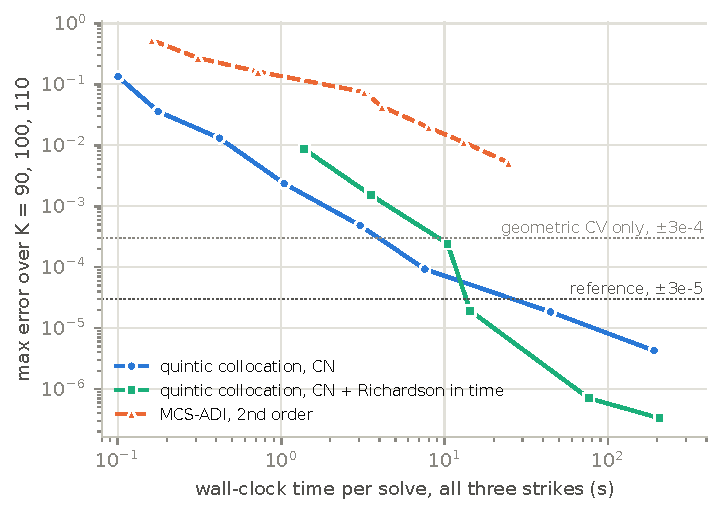
\includegraphics[width=0.8\textwidth]{figs/fig_comparator.pdf}
\caption{Largest error over $K=90,100,110$ against wall-clock time for one solve, arithmetic problem, base
parameters. Errors are relative to the converged collocation price. Horizontal lines mark the uncertainty
of the reference of Table~\ref{tab:ref} and of a Monte Carlo estimate with the geometric control
variate only.}
\label{fig:comparator}
\end{figure}

On the geometric twin the comparison is less one-sided. Its coefficients depend on time, so collocation
has to factorise its system at every step, while ADI only solves banded one-dimensional systems. At the
money, with $N_t=800$, collocation reaches errors of $1.6\times10^{-3}$, $7.3\times10^{-4}$,
$4.1\times10^{-4}$ and $1.8\times10^{-4}$ in 7, 11, 25 and 43 seconds. ADI, with the better of two
clusterings at $v=0$, reaches $1.9\times10^{-2}$, $4.3\times10^{-3}$, $1.8\times10^{-3}$ and
$9.9\times10^{-4}$ in 8, 16, 26 and 36 seconds. Collocation is still ahead at comparable cost, by a factor
of four to twelve, but far less than on the arithmetic problem, where the time-independent operator lets it
factorise once.

The two methods also respond in opposite ways to the clustering of the grid at $v=0$. On the geometric
twin with $N_t=1600$, reducing the clustering width $\alpha_v$ from $0.4$ to $0.005$ lowers the ADI error
at the money from $7.3\times10^{-3}$ to $3.9\times10^{-3}$ ($161\times61$ grid) but raises the collocation
error from $2.4\times10^{-4}$ to $4.3\times10^{-4}$ ($41\times21$ grid). The second-order finite
difference scheme benefits from resolution near the degenerate boundary; the quintic basis does not need it.
How sensitive a solver is to this choice is therefore a property of the method, not only of the problem,
which is worth keeping in mind when results for different Heston schemes are compared.

\subsection{Comparison with published values}\label{sec:published}

\citet{FusaiKyriakou2016} report, in their Table~9, maximal lower bounds for three Heston parameter sets
taken from \citet{EwaldMenkensTing2013}, together with the ADI and Monte Carlo prices of that paper. All
three sets satisfy the Feller condition. Table~\ref{tab:published} puts these numbers next to ours.

\begin{table}[t]
\centering
\caption{Published values for the Heston sets of \citet[Table~1]{EwaldMenkensTing2013}
($S_0=K=100$, $T=1$, $q=0$; set 1: $\kappa=4.75$, $\theta=v_0=0.0483$, $\xi=0.55$, $\rho=-0.569$, $r=0.04$;
set 2: $\kappa=3$, $\theta=v_0=0.1$, $\xi=0.2$, $\rho=0.7$, $r=0.1$; set 3: $\kappa=7$, $\theta=0.05$,
$v_0=0.075$, $\xi=0.3$, $\rho=-0.4$, $r=0.07$) and our results. EMT MC: range of their Monte Carlo
estimates over schemes. Our MC: quadratic-exponential scheme with geometric control variate (2M paths)
and full-truncation Euler without any control variate (16M paths, pooled over 100 to 800 time steps).}
\label{tab:published}
\small
\begin{tabular}{lccc}
\toprule
& set 1 & set 2 & set 3\\
\midrule
\citet{FusaiKyriakou2016}, MLB & 5.854 & 9.323 & 7.123\\
\citet{EwaldMenkensTing2013}, ADI & 5.852839 & 9.323261 & 7.122597\\
\citet{EwaldMenkensTing2013}, MC & 5.851--5.871 & 9.321--9.334 & 7.123--7.136\\
\midrule
MLB, this paper & 5.86532 & 9.32373 & 7.12900\\
MC estimate of the same bound & $5.86510\pm0.00014$ & $9.32409\pm0.00053$ & $7.12889\pm0.00019$\\
MC price, QE with control variate & $5.86576\pm0.00014$ & $9.32549\pm0.00053$ & $7.12949\pm0.00019$\\
MC price, Euler, no control variate & $5.8665\pm0.0019$ & $9.3257\pm0.0035$ & $7.1311\pm0.0024$\\
Collocation & 5.86599 & 9.32513 & 7.12960\\
\bottomrule
\end{tabular}
\end{table}

We could not reproduce the three MLB values. Our bound is higher by $0.0113$, $0.0007$ and $0.0060$, or
$0.19\%$, $0.01\%$ and $0.08\%$ of the price. In practical terms the numbers are close, but on set 1 the
gap is about eighty standard errors of our simulation of the same quantity, so it is not noise. Several
causes can be excluded. Our implementation reproduces Table~10 of the same paper to all printed digits
(Table~\ref{tab:fk10}), is stable under changes of its numerical parameters, and agrees with a direct
simulation of the bound. The optimisation over $\lambda$ cannot explain the gap either, because the bound
is flat near its maximum: even $\lambda=\ln K$, without any optimisation, gives $5.8645$ on set 1. Seven
alternative readings of the parameters (the sign of $\rho$, $\xi$ against $\xi^2$ or $\sqrt\xi$, variance
against volatility for $v_0$ and $\theta$, and the limits $\rho=0$ and $\xi=0$) do not reproduce the table.
Taken over all three sets the reading we use is the closest, although $\rho=0$ comes nearer on set~1 and
$\xi=0$ on set~3. Finally, we simulated the bound itself at our $\lambda^\ast$ with the full-truncation Euler scheme of
\citet{LordKoekkoekvanDijk2010} and no control variate, which shares nothing with our other computations
except the model and the value of $\lambda^\ast$. For set 1 this gives $\LB(\lambda^\ast)=5.8658\pm0.0019$,
six standard errors above the published value. Since any $\LB(\lambda)$ is a lower bound for the maximum,
the published value is not consistent with the model as printed. Two causes we cannot check: how the transform for the continuous average under
Heston was evaluated, since the paper describes this step only in outline, and whether the table was
computed for a specification other than the one printed.

Two observations may help a reader who wants to pursue this. The published bounds agree to three digits
with the ADI prices of \citet{EwaldMenkensTing2013}, which were computed on a uniform grid of 1000 points in
each of $x$, $v$ and $t$, with a Dirichlet condition at $v_{\max}=3$. And the Monte Carlo estimates that
paper reports for set 1 range from $5.851$ to $5.871$ depending on the scheme, a spread wider than the gap
we are discussing. Our collocation price and our two simulations with different schemes agree with each
other within two standard errors of the simulations, and within $6\times10^{-6}$ when the bound is used
as a control variate in the Euler simulation. For the same reason the published values are of limited use
as an external check of a solver. Our collocation prices lie above the published bounds, as they must, but
by a margin that mostly reflects the discrepancy discussed here.

\section{Conclusions}\label{sec:conclusions}

We have described a quintic B-spline collocation method for the continuously monitored arithmetic Asian
call under the Heston model and, with most of the effort, the references needed to check it. The method
is simple to state. It solves the two-dimensional equation obtained from the Rogers--Shi--Ve\v{c}e\v{r}
reduction; the time-independence of that equation lets the whole time march run on two sparse
factorisations; the degenerate boundary $v=0$ is handled by collocating the equation on it; and the price
at any strike is an exact evaluation of the spline.

Against a Monte Carlo reference with a standard error of about $1.6\times10^{-5}$, built from the lower
bound of \citet{FusaiKyriakou2016} used as a control variate, the solver agrees within the reference's
uncertainty at eleven strikes. Over thirteen parameter regimes, including a Feller ratio of $0.08$, the
differences are as large as that uncertainty leads one to expect ($\chi^2=45.6$ for 39 comparisons), once
the domain has been widened where the regime requires it. The
time discretisation is of second order, with a cubic remainder from the Rannacher start-up that two levels
of Richardson extrapolation remove. In space the observed order approaches four from below, the limit of
collocation at Greville points, and the error at a moderate grid of 273 points in $x$ is below
$10^{-6}$. On the same equation and at equal computing time, a modified Craig--Sneyd ADI scheme has an error
about 150 times larger, and within 25 seconds it does not get below $5\times10^{-3}$.

Some results are useful beyond this particular solver. The lower bound of Fusai and Kyriakou can be
computed for the Heston model with a continuous average by two consecutive Riccati integrations, and once
computed it makes an unusually effective control variate. Truncation errors of the computational domain
can be of order $10^{-4}$ while every refinement study looks clean; they showed up only against an
independent reference, at vol-of-vol $\xi=1.5$ and at a five-year maturity. And the published lower bounds
for the Heston cases in \citet{FusaiKyriakou2016} are not consistent with our computations of the same
quantity for the model as printed; we have listed what we could and could not rule out.

The work has limits. We considered one model, one contract and no dividends. The references all rely on
the affine structure of Heston; for a non-affine model the checking strategy would have to change. Our
spatial order is capped at four by the choice of collocation points. For maximally smooth splines there
are two known ways around this cap, moving the points to Galerkin-superconvergent positions
\citep{Anitescu2015,Montardini2017} or keeping them and adding a high-order perturbation of the operator
\citep{IrodotouEllinaHoustis1988,ChristaraNg2006}; classical Gauss-point collocation
\citep{deBoorSwartz1973,BialeckiFairweather2001} would require a less smooth spline space and would lose
the property that the degenerate boundary is a collocation line. None of these has been analysed for a
degenerate operator with a mixed derivative and a kinked terminal condition, and at the accuracy that our
references can confirm there is little to gain yet. Other natural extensions are discrete monitoring,
sensitivities, which the spline representation gives directly, and floating-strike contracts, which the
same reduction covers.


\section*{Code and data availability}
The solver, the reference computations and the scripts that produce every table and figure in this
paper are available at \url{https://github.com/grizzlypuma/heston-asian-collocation} under the MIT
licence. The repository also contains the raw output of all runs in JSON form.

\section*{Use of generative AI}
This work was carried out with substantial help from Claude (Anthropic), an AI assistant. The assistant
wrote most of the code, ran the numerical experiments and the analysis of their results, and drafted the
text of the paper. The author checked the derivations, reran experiments from the repository and compared
them with the reported results, and read and edited the text. The author takes full responsibility for
the content of the paper. Because the code and the raw output of all runs are public, every number in the
paper can be checked independently.

\bibliographystyle{plainnat}
\bibliography{refs}

\appendix
\section{The transform needed for the bound}\label{app:transform}

Fix $t\in[0,T]$ and $\upsilon\in\mathbb C$, write $X=\ln S$ and $c=i\upsilon/T$. Under
\eqref{eq:heston},
\begin{equation*}
\dd X_s = \bigl(r - \tfrac12v_s\bigr)\dd s + \sqrt{v_s}\,\dd W^{(1)}_s,
\end{equation*}
and the quantity we need is
\begin{equation*}
\varphi_t(\upsilon) = \E\bigl[S_t\,e^{i\upsilon Y_T}\bigr]
= \E\Bigl[\exp\Bigl(X_t + c\int_0^T X_u\,\dd u\Bigr)\Bigr].
\end{equation*}

\paragraph{First stage.} For $s\in[t,T]$ let
$g(s,x,v) = \E\bigl[\exp\bigl(c\int_s^TX_u\,\dd u\bigr)\mid X_s=x,\,v_s=v\bigr]$. By the Feynman--Kac
formula, $g$ solves
\begin{equation*}
g_s + \bigl(r-\tfrac v2\bigr)g_x + \kappa(\theta-v)g_v + \tfrac12vg_{xx} + \rho\xi vg_{xv} + \tfrac12\xi^2vg_{vv}
+ c\,x\,g = 0,\qquad g(T,x,v)=1 .
\end{equation*}
The coefficients are affine in $(x,v)$, so we try $g=\exp\bigl(\mathcal A(\tau) + B_x(\tau)x + B_v(\tau)v\bigr)$
with $\tau = T-s$. Dividing by $g$ and collecting the terms that multiply $x$, $v$ and $1$ gives
\begin{equation}\label{eq:appsys}
B_x' = c,\qquad
B_v' = \tfrac12B_x^2 - \tfrac12B_x + \rho\xi B_xB_v + \tfrac12\xi^2B_v^2 - \kappa B_v,\qquad
\mathcal A' = rB_x + \kappa\theta B_v,
\end{equation}
with zero initial values. In particular $B_x(\tau) = c\tau$. Note that the term in $x$ comes only from the
running factor $c\,x$, since no coefficient of the generator depends on $x$; this is what makes $B_x$
linear in $\tau$ and leaves a single Riccati equation, for $B_v$, whose coefficients depend on $\tau$.

\paragraph{Second stage.} By the tower property,
\begin{equation*}
\varphi_t(\upsilon) = \E\Bigl[\exp\Bigl(c\int_0^tX_u\,\dd u\Bigr)
\exp\bigl(\mathcal A(T-t) + (1+B_x(T-t))X_t + B_v(T-t)\,v_t\bigr)\Bigr].
\end{equation*}
This is the same kind of expectation over $[0,t]$ with exponential-affine terminal data, so the same system
\eqref{eq:appsys} applies on $\tau\in[T-t,T]$, started from $\bigl(\mathcal A(T-t),\,1+B_x(T-t),\,B_v(T-t)\bigr)$.
In other words, a single integration of \eqref{eq:appsys} from $\tau=0$ to $\tau=T$ with
$B_x(\tau) = c\tau + \ind\{\tau\ge T-t\}$ does both stages, and
\begin{equation*}
\varphi_t(\upsilon) = \exp\bigl(\mathcal A(T) + (1+i\upsilon)\ln S_0 + B_v(T)\,v_0\bigr).
\end{equation*}
The $B_x$-part of $\mathcal A$ integrates in closed form to $r\bigl(cT^2/2 + t\bigr)$; only the
$\kappa\theta B_v$ part is integrated numerically. Without the jump the same computation returns
$\varphi_0(\upsilon)=\E[e^{i\upsilon Y_T}]$.

\paragraph{Checks.} For $\upsilon=0$ we have $c=0$, $B_x=\ind\{\tau\ge T-t\}$, and the right-hand side of
the $B_v$ equation is $\tfrac12B_x^2-\tfrac12B_x + (\rho\xi B_x-\kappa)B_v + \tfrac12\xi^2B_v^2$, which
vanishes identically for $B_v=0$ whether $B_x$ is zero or one. Hence $B_v\equiv0$, $\mathcal A = rt$, and
$\varphi_t(0)=S_0e^{rt}=\E[S_t]$, as it must be. In the Gaussian limit ($\xi\to0$, $v\equiv\sigma^2$) the pair
$(X_t,Y_T)$ is jointly normal with
\begin{equation*}
\E Y_T = \ln S_0 + \bigl(r-\tfrac{\sigma^2}{2}\bigr)\tfrac T2,\qquad
\operatorname{Var} Y_T = \frac{\sigma^2T}{3},\qquad
\operatorname{Cov}(X_t,Y_T) = \sigma^2\Bigl(t - \frac{t^2}{2T}\Bigr),
\end{equation*}
which gives $\varphi_t$ in closed form and also the bound itself,
\begin{equation*}
\LB(\lambda) = e^{-rT}\Bigl[\frac1T\int_0^T S_0e^{rt}\,
\Phi_{\mathcal N}\Bigl(\frac{\E Y_T + \operatorname{Cov}(X_t,Y_T) - \lambda}{\sqrt{\operatorname{Var}Y_T}}\Bigr)\dd t
- K\,\Phi_{\mathcal N}\Bigl(\frac{\E Y_T-\lambda}{\sqrt{\operatorname{Var}Y_T}}\Bigr)\Bigr],
\end{equation*}
with $\Phi_{\mathcal N}$ the standard normal distribution function. Our Fourier implementation agrees with
this formula to about $10^{-13}$.

\paragraph{Moments.} With $\upsilon = u-i\delta$ the real part of the exponent is $X_t+\delta Y_T$, so the
damping requires $\E[S_te^{\delta Y_T}]<\infty$, a moment of order roughly $1+\delta$. For the Heston model
such moments can explode in finite time when $\rho>0$ and $\xi$ is large. With $\delta=1$ we never observed
a blow-up in the regimes of this paper (it would stop the ODE integrator), and results for
$\delta=0.25$, $0.5$ and $1$ agree.

\section{Numbers behind the figures}\label{app:tables}

\begin{table}[h]
\centering
\caption{Strike profile of Figure~\ref{fig:strikes} (base parameters). Reference: $\MLB+\E[D]$ from
16 million QE paths with 256 steps; collocation: $N_x=392$, $N_v=61$, time-extrapolated.}
\label{tab:strikes}
\small
\begin{tabular}{rccccc}
\toprule
$K$ & collocation & reference & s.e. & difference & diff./s.e.\\
\midrule
80 & 22.0417609 & 22.041784 & $2.9\times10^{-5}$ & $-2.3\times10^{-5}$ & $-0.81$\\
85 & 17.7700973 & 17.770090 & $2.7\times10^{-5}$ & $+0.8\times10^{-5}$ & $+0.28$\\
90 & 13.7602943 & 13.760319 & $2.5\times10^{-5}$ & $-2.5\times10^{-5}$ & $-0.98$\\
95 & 10.1287138 & 10.128698 & $2.4\times10^{-5}$ & $+1.5\times10^{-5}$ & $+0.66$\\
100 & 7.0325232 & 7.032525 & $2.3\times10^{-5}$ & $-0.1\times10^{-5}$ & $-0.06$\\
105 & 4.6303980 & 4.630414 & $2.4\times10^{-5}$ & $-1.6\times10^{-5}$ & $-0.68$\\
110 & 2.9674922 & 2.967497 & $2.5\times10^{-5}$ & $-0.4\times10^{-5}$ & $-0.17$\\
115 & 1.9107425 & 1.910724 & $2.7\times10^{-5}$ & $+1.9\times10^{-5}$ & $+0.70$\\
120 & 1.2578465 & 1.257820 & $2.8\times10^{-5}$ & $+2.7\times10^{-5}$ & $+0.95$\\
125 & 0.8498719 & 0.849871 & $3.0\times10^{-5}$ & $+0.1\times10^{-5}$ & $+0.04$\\
130 & 0.5883959 & 0.588386 & $3.1\times10^{-5}$ & $+1.0\times10^{-5}$ & $+0.31$\\
\bottomrule
\end{tabular}
\end{table}

\begin{table}[h]
\centering
\caption{Parameter regimes of Figure~\ref{fig:regimes}. One parameter differs from the base set.
Domains after the corrections of Section~\ref{sec:regimes}.}
\label{tab:regimes}
\small
\begin{tabular}{llcccr}
\toprule
regime & $K$ & collocation & reference & s.e. & diff./s.e.\\
\midrule
$\rho$=-0.9 & 90 & 14.1367573 & 14.136778 & $2.8\times10^{-5}$ & $-0.74$\\
 & 100 & 6.8626365 & 6.862635 & $1.6\times10^{-5}$ & $+0.07$\\
 & 110 & 1.6255838 & 1.625596 & $1.3\times10^{-5}$ & $-0.95$\\
\addlinespace[2pt]
$\rho$=-0.7 & 90 & 14.0287661 & 14.028814 & $3.5\times10^{-5}$ & $-1.36$\\
 & 100 & 6.9456726 & 6.945708 & $2.9\times10^{-5}$ & $-1.23$\\
 & 110 & 2.1869149 & 2.186932 & $3.1\times10^{-5}$ & $-0.55$\\
\addlinespace[2pt]
$\rho$=-0.3 (base) & 90 & 13.7602892 & 13.760297 & $1.7\times10^{-5}$ & $-0.45$\\
 & 100 & 7.0325248 & 7.032498 & $1.5\times10^{-5}$ & $+1.74$\\
 & 110 & 2.9675003 & 2.967494 & $1.7\times10^{-5}$ & $+0.39$\\
\addlinespace[2pt]
$\rho$=0.0 & 90 & 13.4952725 & 13.495226 & $5.7\times10^{-5}$ & $+0.82$\\
 & 100 & 7.0376366 & 7.037543 & $5.3\times10^{-5}$ & $+1.75$\\
 & 110 & 3.4091524 & 3.409057 & $5.9\times10^{-5}$ & $+1.62$\\
\addlinespace[2pt]
$\rho$=0.5 & 90 & 12.8600662 & 12.860100 & $5.2\times10^{-5}$ & $-0.65$\\
 & 100 & 6.9249363 & 6.924932 & $5.3\times10^{-5}$ & $+0.08$\\
 & 110 & 3.9898051 & 3.989818 & $6.0\times10^{-5}$ & $-0.22$\\
\addlinespace[2pt]
$\rho$=0.9 & 90 & 11.9595001 & 11.959468 & $1.1\times10^{-5}$ & $+2.88$\\
 & 100 & 6.6868654 & 6.686874 & $1.5\times10^{-5}$ & $-0.58$\\
 & 110 & 4.3679011 & 4.367903 & $2.1\times10^{-5}$ & $-0.10$\\
\addlinespace[2pt]
$\xi$=0.3 & 90 & 13.7875111 & 13.787488 & $2.1\times10^{-5}$ & $+1.11$\\
 & 100 & 7.6542525 & 7.654221 & $1.8\times10^{-5}$ & $+1.75$\\
 & 110 & 3.7094223 & 3.709440 & $2.2\times10^{-5}$ & $-0.80$\\
\addlinespace[2pt]
$\xi$=0.6 & 90 & 13.8125316 & 13.812477 & $3.2\times10^{-5}$ & $+1.72$\\
 & 100 & 7.4388835 & 7.438888 & $2.9\times10^{-5}$ & $-0.16$\\
 & 110 & 3.3982489 & 3.398210 & $3.2\times10^{-5}$ & $+1.20$\\
\addlinespace[2pt]
$\xi$=1.5 & 90 & 13.6238358 & 13.623934 & $7.6\times10^{-5}$ & $-1.28$\\
 & 100 & 6.5072983 & 6.507197 & $6.9\times10^{-5}$ & $+1.46$\\
 & 110 & 2.5281128 & 2.528089 & $7.6\times10^{-5}$ & $+0.31$\\
\addlinespace[2pt]
T=0.25 & 90 & 10.9207922 & 10.920802 & $0.8\times10^{-5}$ & $-1.29$\\
 & 100 & 3.5392539 & 3.539259 & $0.6\times10^{-5}$ & $-0.81$\\
 & 110 & 0.5513522 & 0.551359 & $0.7\times10^{-5}$ & $-0.87$\\
\addlinespace[2pt]
T=0.5 & 90 & 12.0098385 & 12.009846 & $2.0\times10^{-5}$ & $-0.38$\\
 & 100 & 4.9813995 & 4.981400 & $1.7\times10^{-5}$ & $-0.03$\\
 & 110 & 1.4240131 & 1.424042 & $2.0\times10^{-5}$ & $-1.41$\\
\addlinespace[2pt]
T=3.0 & 90 & 18.5491752 & 18.549276 & $12.5\times10^{-5}$ & $-0.80$\\
 & 100 & 12.5357125 & 12.535728 & $11.4\times10^{-5}$ & $-0.13$\\
 & 110 & 7.9780757 & 7.978155 & $11.3\times10^{-5}$ & $-0.70$\\
\addlinespace[2pt]
T=5.0 & 90 & 21.9991610 & 21.999016 & $19.4\times10^{-5}$ & $+0.75$\\
 & 100 & 16.5503620 & 16.550151 & $17.9\times10^{-5}$ & $+1.18$\\
 & 110 & 12.0954212 & 12.095376 & $17.3\times10^{-5}$ & $+0.26$\\
\addlinespace[2pt]
\bottomrule
\end{tabular}
\end{table}

\begin{table}[h]
\centering
\caption{Runs of Figure~\ref{fig:comparator}. Errors relative to the converged collocation price;
time for one solve (three solves for the extrapolated variant).}
\label{tab:comp}
\footnotesize\setlength{\tabcolsep}{4pt}
\begin{tabular}{llrccc}
\toprule
method & grid & time (s) & error $K=90$ & error $K=100$ & error $K=110$\\
\midrule
colloc., CN & $35\times21$, $N_t=200$ & 0.10 & $1.2\times10^{-1}$ & $4.6\times10^{-2}$ & $1.3\times10^{-1}$\\
colloc., CN & $52\times21$, $N_t=400$ & 0.18 & $1.0\times10^{-2}$ & $7.2\times10^{-3}$ & $3.6\times10^{-2}$\\
colloc., CN & $69\times31$, $N_t=400$ & 0.42 & $6.1\times10^{-3}$ & $4.9\times10^{-3}$ & $1.3\times10^{-2}$\\
colloc., CN & $103\times31$, $N_t=800$ & 1.05 & $5.6\times10^{-4}$ & $9.3\times10^{-4}$ & $2.4\times10^{-3}$\\
colloc., CN & $137\times41$, $N_t=1600$ & 3.05 & $3.9\times10^{-5}$ & $9.6\times10^{-5}$ & $4.8\times10^{-4}$\\
colloc., CN & $188\times41$, $N_t=3200$ & 7.58 & $1.2\times10^{-5}$ & $2.3\times10^{-5}$ & $9.3\times10^{-5}$\\
colloc., CN & $273\times61$, $N_t=6400$ & 44.61 & $2.2\times10^{-6}$ & $9.9\times10^{-6}$ & $1.8\times10^{-5}$\\
colloc., CN & $392\times61$, $N_t=12800$ & 191.43 & $5.6\times10^{-7}$ & $2.6\times10^{-6}$ & $4.3\times10^{-6}$\\
\addlinespace[2pt]
colloc., CN+extrap. & $69\times31$, $N_t=200/400/800$ & 1.38 & $5.5\times10^{-3}$ & $7.5\times10^{-3}$ & $8.7\times10^{-3}$\\
colloc., CN+extrap. & $103\times31$, $N_t=400/800/1600$ & 3.53 & $3.6\times10^{-4}$ & $1.5\times10^{-3}$ & $1.2\times10^{-3}$\\
colloc., CN+extrap. & $137\times41$, $N_t=800/1600/3200$ & 10.43 & $8.6\times10^{-5}$ & $2.4\times10^{-4}$ & $1.9\times10^{-4}$\\
colloc., CN+extrap. & $188\times41$, $N_t=800/1600/3200$ & 14.35 & $7.5\times10^{-7}$ & $1.4\times10^{-5}$ & $1.9\times10^{-5}$\\
colloc., CN+extrap. & $273\times61$, $N_t=1600/3200/6400$ & 76.17 & $7.1\times10^{-7}$ & $6.3\times10^{-7}$ & $3.4\times10^{-9}$\\
colloc., CN+extrap. & $392\times61$, $N_t=1600/3200/6400$ & 206.77 & $1.8\times10^{-7}$ & $3.2\times10^{-7}$ & $3.3\times10^{-7}$\\
\addlinespace[2pt]
MCS-ADI & $81\times31$, $N_t=400$ & 0.16 & $5.3\times10^{-1}$ & $2.3\times10^{-2}$ & $5.3\times10^{-1}$\\
MCS-ADI & $121\times41$, $N_t=400$ & 0.31 & $2.4\times10^{-1}$ & $6.4\times10^{-2}$ & $2.7\times10^{-1}$\\
MCS-ADI & $161\times41$, $N_t=800$ & 0.72 & $1.1\times10^{-1}$ & $7.0\times10^{-2}$ & $1.6\times10^{-1}$\\
MCS-ADI & $241\times61$, $N_t=1600$ & 3.22 & $3.4\times10^{-2}$ & $4.8\times10^{-2}$ & $7.5\times10^{-2}$\\
MCS-ADI & $321\times61$, $N_t=1600$ & 4.15 & $1.8\times10^{-2}$ & $3.0\times10^{-2}$ & $4.3\times10^{-2}$\\
MCS-ADI & $481\times81$, $N_t=1600$ & 8.01 & $8.1\times10^{-3}$ & $1.4\times10^{-2}$ & $2.0\times10^{-2}$\\
MCS-ADI & $641\times101$, $N_t=1600$ & 13.13 & $4.3\times10^{-3}$ & $7.4\times10^{-3}$ & $1.1\times10^{-2}$\\
MCS-ADI & $961\times121$, $N_t=1600$ & 24.59 & $1.4\times10^{-3}$ & $3.0\times10^{-3}$ & $5.2\times10^{-3}$\\
\addlinespace[2pt]
\bottomrule
\end{tabular}
\end{table}


\end{document}
